\documentclass[11pt,a4paper]{article}
\usepackage[margin=23mm,headheight=15pt]{geometry}
\usepackage{fontspec}
\setmainfont{Noto Serif CJK KR}[ItalicFont={Noto Serif CJK KR},ItalicFeatures={FakeSlant=0.15}]
\setsansfont{Noto Sans CJK KR}
\setmonofont{DejaVu Sans Mono}[Scale=0.78]
\XeTeXlinebreaklocale "ko"
\XeTeXlinebreakskip=0pt plus 0.1em
\usepackage{amsmath,amssymb,booktabs,longtable,tabularx,array,graphicx,caption,xcolor,xurl,enumitem,fancyhdr}
\usepackage[unicode,colorlinks=true,linkcolor=blue!45!black,urlcolor=blue!55!black,citecolor=blue!45!black]{hyperref}
\usepackage{setspace}
\setstretch{1.22}
\setlength{\parindent}{0pt}
\setlength{\parskip}{6pt}
\setlength{\emergencystretch}{2em}
\renewcommand{\figurename}{그림}
\renewcommand{\tablename}{표}
\renewcommand{\refname}{참고문헌}
\captionsetup{font=small,labelfont=bf}
\pagestyle{fancy}
\fancyhf{}
\fancyhead[L]{\small\sffamily TRADEGEN · Retrospective Strategy Research}
\fancyhead[R]{\small\sffamily 2026-10-31}
\fancyfoot[C]{\small\thepage}
\title{\sffamily\bfseries 대규모 규칙 기반 전략 탐색에서\break 비용과 선택편향의 영향\\[5pt]\large Costs, Selection Bias, and the Limits of Broad Strategy Search}
\author{TRADEGEN Research\\\small Computational research report prepared with Codex}
\date{2026년 10월 31일 · 재현 가능한 회고적 연구보고서}
\begin{document}
\maketitle
\thispagestyle{empty}
\begin{center}\small\textbf{연구 상태: 회고적 탐색 분석 / 비심사 보고서 / 실거래 검증 아님}\end{center}
\begin{abstract}
We evaluate 21,408 asset--configuration pairs across eight economic rule families and eight asset price series. A frozen protocol uses 2021--2022 for selection and 2023--September 2026 for an internal holdout, with next-close execution, fee-inclusive self-financing ledgers, and a costed buy-and-hold benchmark. Centered joint block-bootstrap maximum-mean tests and Holm correction address the declared search multiplicity. The selection rule retains 6 asset-level candidates; 4 have positive internal-holdout mean returns. 0 asset-level validation omnibus tests and 0 selected-versus-benchmark holdout tests meet the adjusted 5\% threshold; 0 candidates satisfy all preregistered exploratory conditions. These counts distinguish positive absolute performance from benchmark-relative evidence. Because the historical caches were previously inspected, the results are retrospective diagnostics, not independent confirmation. Close-only fractional-capital simulations do not validate executable limit fills, realized account profit, principal protection, or production deployment.
\end{abstract}
\textbf{국문 초록.} 여덟 경제적 규칙군과 여덟 가격 시계열에서 21,408개 자산·설정 조합을 평가하였다. 2021--2022년을 선택 구간으로, 2023년부터 2026년 9월까지를 회고적 내부 이후 구간으로 고정하였다. 다음 종가 실행, 비용 포함 자기금융 장부, 비용 차감 단순 보유와의 비교, 공동 블록 재표본화와 Holm 보정을 적용하였다. 선택된 6개 중 이후 구간 평균수익이 양수인 것은 4개이다. 보정 5\% 수준에서 검증 전체 집합은 0개 자산, 고정 선택의 이후 구간 벤치마크 우위는 0개 자산이며, 사전 명시한 탐색 조건을 모두 만족한 것은 0개이다. 이미 사용한 가격 캐시와 소수 수량·종가 모형이라는 한계 때문에 이 결과를 독립 확인이나 실거래 승인으로 해석하지 않는다.

\textbf{핵심어:} 시계열 모멘텀, 평균회귀, 변동성 관리, 거래비용, 데이터 스누핑, 다중검정, 내부 표본외 평가.

본 보고서는 공개 가격 캐시의 계산 결과와 그 한계를 설명한다. 연구상의 정규화 자산은 실제 계좌의 실현 순이익이 아니며, 보고서의 결론은 주문·세션 활성화 또는 원금 보장에 대한 승인이 아니다.

\section{서론: 후보를 많이 만들면 무엇이 늘어나는가}
전략의 수를 늘리면 유용한 가설을 놓칠 가능성은 줄어들지만 우연히 좋은 과거 성적을 얻을 기회도 함께 늘어난다. 같은 가격에서 계산한 이동평균, 추세, 돌파 규칙은 경제적으로 겹치고 수익률도 강하게 상관된다. 따라서 후보 수를 독립적인 발견 수로 세거나, 최상위 백테스트 하나를 보여주는 방식은 연구 질문에 답하지 못한다. 본 연구의 질문은 \emph{다수의 사전 고정 규칙을 동일한 비용·시차·선택 절차로 비교했을 때, 어떤 성과가 단순 보유와 비교해 남으며 어느 주장이 아직 입증되지 않는가}이다.

분석은 가격 지속성과 반전을 묻는 여덟 규칙군에 공통 실행 변형을 결합한다. 신호의 경제적 설명, 계좌 안에서의 실현 가능성, 통계적 유의성은 별개이다. 반등을 잡는 규칙이 과거에 수익을 냈다는 사실만으로 투자자의 과잉반응을 식별할 수 없고, 최대 낙폭을 줄였다는 사실만으로 초과수익을 만들었다고 결론낼 수도 없다. 전체 후보와 실패를 함께 공개하고, 탐색 구간에서 결정한 선택을 이후 구간에 고정하여 이 구분을 유지한다.

본 연구의 자료는 이전 연구에서 이미 관찰된 캐시이다. 2023년 이후 구간은 이번 선택 알고리즘에 넣지 않았지만, 완전히 새로운 정보 또는 사전 봉인된 확인 표본은 아니다. 이후 모든 ``검증'' 표현은 이 회고적 내부 평가를 뜻한다. 기존 S\_C3 연구의 PASS 판정은 이 후보 집합이나 새로운 위험 정책으로 승계하지 않는다.

\section{경제적 가설과 관련 문헌}
\subsection{추세와 정보의 점진적 반영}
시계열 모멘텀은 과거 수익률의 부호나 크기가 미래 방향과 관련되는지를 묻는다. 정보의 느린 반영, 투자 흐름의 지속, 위험 프리미엄의 변화는 가능한 설명이지만 가격 규칙만으로 어느 설명이 맞는지는 구별할 수 없다. Moskowitz, Ooi, Pedersen의 연구\cite{tsmom}는 이 가설의 주요 근거이나, 그 선물 포트폴리오와 본 연구의 단일 현물 매수·현금 규칙은 자산, 레버리지, 공매도, 비용에서 다르다.

이동평균과 거래 범위 돌파는 같은 지속성 가설의 다른 표현이다\cite{technical}. 긴 창은 잡음을 줄이는 대신 전환에 늦고, 짧은 창은 빠르게 반응하는 대신 비용이 커질 수 있다. 창 길이·진입 여유·재조정 주기를 바꾸는 일은 새로운 경제 이론을 만드는 일이 아니라 같은 가설의 민감도와 구현 선택을 탐색하는 일이다.

\subsection{평균회귀와 유동성 제공}
표준화 가격 편차, RSI, 최근 고점 대비 하락률은 단기 반전을 가정하는 규칙을 제공한다. 일시적 주문 불균형이나 유동성 수요가 가격에 영향을 준다면 역방향 거래에 보상이 생길 수 있지만, 하락이 정보 변화라면 반등을 기다리는 포지션은 손실을 확대한다. Lo와 MacKinlay\cite{contrarian}가 보인 것처럼 역추세 수익이 곧 과잉반응의 증거는 아니다. 본 연구의 단일 자산 규칙은 그 논문의 횡단면 전략을 재현하지 않으며, 경제적 설명은 검증 대상 가설로만 취급한다.

\subsection{변동성 상태와 위험 조절}
변동성이 높을 때 기대수익이 위험과 정확히 비례해 증가하지 않는다면 위험을 낮추는 정책이 위험조정 성과를 바꿀 수 있다\cite{volmanaged}. 본 연구는 차입 없이 목표 노출을 제한하는 변형을 비교한다. 따라서 원 논문의 역분산 요인 포트폴리오와 동일하지 않다. 변동성 관리는 방향 예측과 구별되며, 평균 노출이 낮아져 낙폭과 수익률이 함께 감소하는 결과도 경제적으로 자연스럽다.

추세 전략의 급격한 회복 국면 위험을 다룬 문헌\cite{crashes}은 평균 샤프비율 외에 경로와 꼬리를 확인해야 함을 보여준다. 다만 원래의 롱숏 모멘텀 붕괴 메커니즘을 본 현물 매수·현금 규칙에 그대로 적용하지 않는다. 표본별 자산곡선, 최대 낙폭, 비용 스트레스, 시차 민감도를 함께 보고 이 구분을 유지한다.

\subsection{경제적 성과와 발견 오류}
많은 후보 중 최고 성적은 우연과 실제 예측력을 함께 포함한다. 금융 변수 탐색의 다중성 문제\cite{factorzoo}를 단일 후보의 보통 $p$값으로 해결할 수 없다. 본 연구는 전체 선언 후보의 최대 통계량을 공동 재표본화하는 White 계열의 접근\cite{white}을 사용한다. 이는 Hansen의 SPA 검정\cite{hansen}을 구현했다는 뜻이 아니며, 나쁜 후보까지 중심화하는 보수적 방법임을 명시한다.

\section{자료와 사전 고정 실험 설계}
\subsection{자료 출처와 품질}
자료 목록의 46개 파일 중 사전에 정한 여덟 시계열만 사용하였다. 미국 ETF 네 개, 한국 지수 ETF 한 개, 원화 비트코인 및 USDT 표시 비트코인·이더리움이 포함된다. 종가와 날짜 이외의 호가·체결·거래량 정보는 없다. 고정 마감일은 2026-09-24이며 한국 ETF의 마지막 관측은 2026-09-23이다. 모든 선택 캐시는 2026-09-27의 이전 자산 확장 연구에 이미 사용되었다. 2026-10-31 작성 시점의 실시간 가격 또는 최신 계좌 상태를 조회한 자료가 아니다.
\begin{table}[htbp]\centering
\small
\setlength{\tabcolsep}{4pt}
\caption{선택 자료와 표시 통화}
\begin{tabular}{llccr}
\toprule
자산 & 통화 & 최초 일자 & 최종 일자 & 사용 행 수 \\
\midrule
SPY & USD & 1995-01-03 & 2026-09-24 & 7,985 \\
QQQ & USD & 1999-03-10 & 2026-09-24 & 6,929 \\
GLD & USD & 2004-11-18 & 2026-09-24 & 5,496 \\
TLT & USD & 2002-07-30 & 2026-09-24 & 6,078 \\
TIGER200 & KRW & 2009-04-17 & 2026-09-23 & 4,266 \\
BTC\_KRW & KRW & 2017-09-25 & 2026-09-24 & 3,287 \\
BTC\_USDT & USDT & 2017-08-17 & 2026-09-24 & 3,326 \\
ETH\_USDT & USDT & 2017-08-17 & 2026-09-24 & 3,326 \\
\bottomrule
\end{tabular}
\par\smallskip\begin{minipage}{\linewidth}\footnotesize 사용 행 수는 고정 마감일 이후 행을 제거한 뒤, 공통 500봉 준비 구간을 제거하기 전이다. 전체 파일·선택 행의 지문은 데이터 매니페스트에 보관한다.\end{minipage}
\end{table}

모든 선택 파일은 날짜가 증가하고 중복 날짜가 없으며 양의 유한 종가를 가진다. Yahoo 계열의 공급자 조정 종가는 독립적으로 감사한 총수익 자료나 당시 시점의 기업행동 빈티지가 아니다. 현금 배당을 별도로 더하지 않는다. 암호자산의 일자는 UTC 캔들 기준이며, Upbit 일봉은 서울 09:00 경계와 관련된다. 캡처 시각이 보존되지 않아 마지막 저장 일자를 제거한 것은 보수적 규칙일 뿐, 모든 봉의 마감 상태를 독립 인증한 것은 아니다.

KODEX 200 초기 자료의 800일 공백은 단순히 채워 넣지 않고, 그 시계열을 제외하고 TIGER 200을 선택한 사유로 기록하였다. 다른 휴장일 간격을 모두 오류로 간주하지도 않았다. 현재 빈티지·결측치가 있는 거시 시계열은 예측 입력에서 제외하였다. 따라서 본 연구는 가격 기반 기술 규칙 연구이며 거시경제 지표의 시점 정합성을 검증한 연구가 아니다.

\subsection{시간 분리와 선택 고정}
\begin{table}[htbp]\centering
\small
\setlength{\tabcolsep}{4pt}
\caption{자산별 실제 평가 행 수}
\begin{tabular}{lrrr}
\toprule
자산 & 2020년까지 & 2021--2022 & 2023년 이후 \\
\midrule
SPY & 6,047 & 503 & 935 \\
QQQ & 4,991 & 503 & 935 \\
GLD & 3,558 & 503 & 935 \\
TLT & 4,140 & 503 & 935 \\
TIGER200 & 2,385 & 490 & 891 \\
BTC\_KRW & 694 & 730 & 1,363 \\
BTC\_USDT & 733 & 730 & 1,363 \\
ETH\_USDT & 733 & 730 & 1,363 \\
\bottomrule
\end{tabular}
\par\smallskip\begin{minipage}{\linewidth}\footnotesize 각 시계열 최초 500봉은 신호 준비에 사용하고 평가에서 제외하였다. 최소 행 기준은 각각 500/365/365이다.\end{minipage}
\end{table}
학습이라고 표시한 2020년까지의 구간은 규칙 진단 구간이며 추정형 모형을 적합하거나 그 성적으로 후보를 고르지 않는다. 모든 규칙과 매개변수는 수익 평가 전 코드·카탈로그·프로토콜과 함께 고정되었다. 2021-01-01--2022-12-31에 선택을 끝내고 선택 레지스트리를 저장한 뒤 2023-01-01--2026-09-24를 평가하였다.

각 구간은 현금에서 시작하고 마지막 관측에서 비용을 납부하며 청산한다. 가격 이력은 신호 계산에 사용할 수 있지만 이후 구간의 수익률은 선택 목적함수에 들어가지 않는다. 모든 후보의 이후 구간 성적을 보조 CSV에 남기는 것은 사후 진단을 위한 것이며, 그 결과를 다시 골라 최종 전략이라고 선언하지 않는다. 이미 알려진 자료라는 오염은 시간 분리로 사라지지 않으므로, 유의한 결과도 장래 확인 실험을 요구하는 탐색 증거이다.

\section{후보 생성, 실행 및 평가 모형}
\subsection{여덟 가설군과 전체 탐색 규모}
\begin{table}[htbp]\centering
\small
\setlength{\tabcolsep}{4pt}
\caption{경제적 가설군과 자산당 탐색 크기}
\begin{tabular}{lrr}
\toprule
규칙군 & 기본 규칙 & 실행 변형 포함 \\
\midrule
시계열 모멘텀 & 27 & 324 \\
단일 이동평균 & 27 & 324 \\
이동평균 교차 & 40 & 480 \\
이전 범위 돌파 & 15 & 180 \\
가격 표준점수 반전 & 30 & 360 \\
RSI 반전 & 30 & 360 \\
저변동성 추세 & 27 & 324 \\
고점 하락 후 반전 & 27 & 324 \\
합계 & 223 & 2,676 \\
\bottomrule
\end{tabular}
\end{table}
223개 기본 규칙에 1·5·21봉 재조정, 목표 비중 상한 0.5·1.0, 변동성 목표 없음·연 15\%를 교차하여 자산당 2,676개를 만든다. 변동성 목표가 있으면 과거 20봉의 연환산 변동성으로 목표 비중을 정하고 상한을 적용한다. 선언한 자산·설정은 21,408개이며 실제 평가한 수는 21,408개이다. 이는 서로 독립적인 전략 2만여 개를 발견했다는 뜻이 아니다. 매개변수 전체와 후보 ID는 카탈로그와 전체 결과 CSV에 기록한다.

추세 규칙은 과거 수익률, 이동평균, 단기·장기 평균의 상대 위치 또는 이전 거래 범위의 이탈을 사용한다. 반전 규칙은 로그가격 표준점수, 단순 이동평균 방식의 상승·하락 폭으로 만든 RSI, 최근 고점 대비 하락과 회복을 사용한다. 저변동성 추세는 과거 변동성 분위수와 양의 모멘텀을 동시에 요구한다. RSI는 Wilder 평활식으로 바꿔 해석하지 않는다. 모든 신호는 해당 시점까지의 자료만 이용하고, 거래 범위는 현재 가격을 제외한 과거 창과 비교한다.

\subsection{자기금융 현금·주식 장부}
종가 $P_t$에서 거래 직전 현금 $C_t$와 수량 $q_t$가 주어지면
\begin{equation}
 E_t^- = C_t + q_tP_t,\qquad V_t=q_tP_t.
\end{equation}
비용률 $c$와 거래 후 목표 비중 $w_t$를 동시에 만족하도록 매수·매도 명목액을 다음과 같이 계산한다.
\begin{equation}
 B_t=\frac{\max(w_tE_t^- - V_t,0)}{1+cw_t},\qquad
 S_t=\frac{\max(V_t-w_tE_t^-,0)}{1-cw_t}.
\end{equation}
\begin{equation}
 C_t^+=C_t+S_t-B_t-c(B_t+S_t),\quad
 q_t^+=q_t+(B_t-S_t)/P_t,\quad
 R_t=\frac{C_t^++q_t^+P_t}{E_{t-1}^+}-1.
\end{equation}
현금과 수량의 비음수성 및 차입 없는 노출을 확인한다. 재조정일 사이에는 수량을 고정하므로 가격 변화로 비중이 표류할 수 있다. 설정한 비중 상한은 재조정 목표의 상한이며 모든 순간의 비중 상한이라고 표현하지 않는다. 거래회전은 단순 목표 비중 차이가 아니라 거래 명목액 $(B_t+S_t)/E_t^-$이므로 표류한 비중을 되돌리는 거래도 비용을 부담한다.

신호를 관측한 종가 $t$에서 즉시 체결시키지 않고 $t+1$ 종가에서 실행한 다음 그 이후의 가격 변화만 수익으로 인식한다. 추가 지연 스트레스에서는 $t+2$ 종가를 사용한다. 이는 일봉 종가 실행 가정이며, 실제 지정가 체결 가능성의 증명은 아니다. 현금 이자는 0이고, 소수 단위 수량을 허용하는 정규화 모형이므로 정수 주식·최소 주문금액·세금·환전·결제 제약은 별도의 실계좌 모형이 필요하다.

\begin{table}[htbp]\centering
\small
\setlength{\tabcolsep}{4pt}
\caption{거래비용 가정: 거래 명목액 대비 편도 bp}
\begin{tabular}{lrrr}
\toprule
자산군 & 기본 & 2배 & 3배 \\
\midrule
미국 ETF & 50 & 100 & 150 \\
한국 지수 ETF & 3 & 6 & 9 \\
암호자산 & 10 & 20 & 30 \\
\bottomrule
\end{tabular}
\par\smallskip\begin{minipage}{\linewidth}\footnotesize 1 bp = 0.01\%. 기존 연구 비용 하한에서 고정한 모형 가정이며 현재 중개사 요율표가 아니다.\end{minipage}
\end{table}
단순 보유 벤치마크도 같은 구간의 첫 매수·마지막 매도 비용을 납부한다. 비용은 보고된 계좌 요율이 아니라 고정 연구 가정이며, 실제 세금과 시장 충격을 모두 포함했다고 주장하지 않는다. 2배·3배 비용과 추가 한 봉 지연을 별도로 평가하며, 이 민감도로 후보를 다시 선택하지 않는다.

\subsection{성과 지표와 선택 규칙}
연환산 계수 $A$는 ETF에 252, 암호자산에 365를 사용한다. 현금수익률이 0인 모형에서 $\widehat{SR}=\sqrt{A}\bar R/s_R$이고, $\widehat{CAGR}=(\prod_t(1+R_t))^{A/n}-1$이다. 최대 낙폭은 최초 자산 1을 포함한 누적 고점에 대한 하락률이며, 매수·매도 거래비용을 포함한다. 연환산은 비교 관례이지 동일한 거래 시간대나 계좌 통화라는 의미가 아니다.

검증 구간에서 비용 차감 평균수익이 양수이고 완결된 왕복 거래가 20회 이상인 후보 중 샤프비율이 가장 높은 하나를 자산별로 고정한다. 허용 오차 안의 동률은 낮은 회전율, 그다음 고정 후보 ID로 결정한다. 자격 후보가 없으면 무조건 하나를 고르지 않고 선택 없음으로 남긴다. 후보 ID는 설정 내용에 결합되며, 이후 구간 결과를 본 뒤 바꾸지 않는다.

\section{통계적 검증과 해석 범위}
\subsection{전체 후보 집합에 대한 최대 통계량}
자산별 검증 구간에서 후보 $j$의 비용 차감 수익률과 동일 비용 단순 보유 수익률의 차이를 $d_{tj}=R_{tj}-R_{t,BH}$로 둔다. 귀무가설은 선언한 후보 집합에서 양의 평균 초과수익을 가진 후보가 없다는 것이다. 관측 통계량은
\begin{equation}
 T=\max\{0,\sqrt{n}\max_j\bar d_j\}.
\end{equation}
각 후보를 자신의 표본평균으로 중심화한 뒤, 모든 후보에 같은 원형 이동 블록 표본을 적용하여 횡단 후보 상관과 시계열 의존을 함께 보존한다. 주 분석은 블록 길이 20, 반복 1,999회이며 길이 5·60에서 각 999회로 민감도를 확인한다. 블록 재표본화의 근거는 의존 관측에 대한 부트스트랩 문헌\cite{kunsch}에 있으나, 구조 변화와 비정상성이 큰 자료에서 유한 표본의 정확성을 보장하지 않는다.

해석에는 선택한 블록이 의존 구조를 충분히 담고 과정이 대략 약정상적이라는 가정이 필요하다. 드문 진입·종료 비용 충격, 상태 전환, 두 해에 불과한 선택 표본은 검정의 보정 정확도를 제한한다. 블록 길이별 원시 $p$값을 함께 공개하며 유리한 길이로 통과 여부를 바꾸지 않는다.

몬테카를로 $p$값은 $(1+\#\{T_b^*\ge T\})/(B+1)$로 계산한다. 유한 반복에서 가능한 최소 해상도를 명시하고 $p=0$으로 표시하지 않는다. 모든 후보를 중심화하는 이 검정은 나쁜 후보의 존재로 보수적일 수 있다. 비유의 결과는 모든 예측 가능성이 없다는 증명이 아니며, 검정 설계와 표본에서 주장할 증거가 부족하다는 결론이다.

\subsection{자산 간 보정과 고정 선택의 이후 구간}
여덟 자산의 전체 집합 검정에는 Holm 순차 보정\cite{holm}을 적용한다. 이미 고정된 자산별 선택의 이후 구간에서도 단순 보유 대비 평균수익 차이를 쌍별 블록 부트스트랩(20봉, 1,999회)으로 분석하고 자산 간 Holm 보정을 적용한다. 양의 절대수익과 단순 보유 대비 우위는 다른 귀무가설이므로 혼동하지 않는다. 차이의 개별 95\% 백분위 신뢰구간과 원시·보정 $p$값을 함께 제시한다. 신뢰구간 자체를 동시 95\% 구간이라고 부르지 않는다.

보조적으로 $R_t=\alpha+\beta R_{t,BH}+u_t$ 시장모형의 절편과 Bartlett 가중 Newey--West HAC 표준오차\cite{neweywest}를 제시한다. 시차는 20, 유한 표본 공분산 보정은 $n/(n-2)$이며 정규 근사의 단측 $p$값을 진단용으로 표시한다. 이는 시장 노출을 줄인 효과와 잔여 관계를 설명하는 진단이며, 요인 전체를 통제한 구조적 알파, 인과효과 또는 독립 확인 결과가 아니다. 사후 선택 후보의 검정 오차와 과거 자료 재사용 문제를 이 회귀가 제거하지 않는다.

사전 고정한 \texttt{promising\_exploratory} 표지는 다음 다섯 조건을 모두 요구한다. 검증 전체 집합의 Holm 보정 $p\le0.05$, 고정 선택의 이후 구간 단순 보유 대비 평균 차이의 Holm 보정 $p\le0.05$, 이후 구간 비용 차감 평균수익 양수, 2배 비용에서 평균수익 양수, 이후 구간 완결 왕복 거래 30회 이상이다. 어느 조건이든 빠지면 사전 기준을 통과했다고 부르지 않는다. 모두 충족하더라도 자료 재사용과 실행 제약 때문에 실거래 검증으로 승격하지 않는다.

\section{실증 결과}
총 21,408개 조합이 결과 CSV에 기록되었고 자산별 6개 선택을 고정하였다. 검증 구간 전체 후보 검정에서 Holm 보정 5\% 수준을 통과한 자산은 0개, 고정 선택의 이후 구간 단순 보유 대비 평균수익 검정을 통과한 자산은 0개이다. 다섯 탐색 조건을 모두 만족한 선택은 0개이며, 어떤 경우에도 실거래 인증을 부여하지 않는다.
\begin{table}[htbp]\centering
\footnotesize
\setlength{\tabcolsep}{4pt}
\caption{사전 고정 추론과 탐색 조건}
\begin{tabular}{lrrrrr}
\toprule
자산 & 검증 원시 $p$ & 검증 Holm & 이후 원시 $p$ & 이후 Holm & 전체 조건 \\
\midrule
SPY & 0.7675 & 1.0000 & 1.0000 & 1.0000 & 미충족 \\
QQQ & 0.4920 & 1.0000 & 1.0000 & 1.0000 & 미충족 \\
GLD & 0.6420 & 1.0000 & -- & 1.0000 & 미충족 \\
TLT & 0.0680 & 0.5440 & -- & 1.0000 & 미충족 \\
TIGER200 & 0.0920 & 0.6440 & 0.9890 & 1.0000 & 미충족 \\
BTC\_KRW & 0.3655 & 1.0000 & 0.9880 & 1.0000 & 미충족 \\
BTC\_USDT & 0.4965 & 1.0000 & 0.9980 & 1.0000 & 미충족 \\
ETH\_USDT & 0.7665 & 1.0000 & 0.8605 & 1.0000 & 미충족 \\
\bottomrule
\end{tabular}
\par\smallskip\begin{minipage}{\linewidth}\footnotesize 검증은 전체 후보 집합의 최대 평균 초과수익 검정이다. 이후 구간은 고정 선택의 단순 보유 대비 평균 차이 검정이다. 결측 검정은 Holm 계열에서 1로 처리한다.\end{minipage}
\end{table}
\begin{table}[htbp]\centering
\footnotesize
\setlength{\tabcolsep}{4pt}
\caption{이후 구간 초과수익과 시장모형 진단}
\begin{tabular}{lrrrr}
\toprule
자산 & 일평균 차이 bp & 차이 95\% CI & HAC $\alpha$ bp/일 & 진단 $p$ \\
\midrule
SPY & -9.02 & [-12.49, -5.62] & -5.37 & 0.9999 \\
QQQ & -13.42 & [-19.50, -7.84] & -5.75 & 0.9990 \\
GLD & -- & -- & -- & -- \\
TLT & -- & -- & -- & -- \\
TIGER200 & -12.28 & [-22.81, -2.02] & -2.61 & 0.7513 \\
BTC\_KRW & -12.45 & [-23.60, -1.60] & 0.12 & 0.4627 \\
BTC\_USDT & -14.44 & [-24.99, -4.34] & -4.31 & 0.9340 \\
ETH\_USDT & -8.63 & [-23.79, 6.84] & 1.61 & 0.1628 \\
\bottomrule
\end{tabular}
\par\smallskip\begin{minipage}{\linewidth}\footnotesize 차이는 선택 수익률에서 비용 차감 단순 보유 수익률을 뺀 값이다. 신뢰구간은 다중성 보정 전 개별 쌍별 블록 부트스트랩 구간이다. HAC 절편 검정은 진단용 원시 단측 p이며 본 연구의 통과 조건이 아니다.\end{minipage}
\end{table}
\begin{table}[htbp]\centering
\footnotesize
\setlength{\tabcolsep}{4pt}
\caption{검증 블록 길이 민감도와 선택 가능한 후보}
\begin{tabular}{lrrrrr}
\toprule
자산 & $p$: 5봉 & $p$: 20봉 & $p$: 60봉 & 자격 후보 수 & 서로 다른 경로 \\
\midrule
SPY & 0.7830 & 0.7675 & 0.7260 & 1 & 1845 \\
QQQ & 0.5250 & 0.4920 & 0.3890 & 9 & 1986 \\
GLD & 0.6470 & 0.6420 & 0.6270 & 0 & 1761 \\
TLT & 0.0460 & 0.0680 & 0.1060 & 0 & 1657 \\
TIGER200 & 0.1020 & 0.0920 & 0.0440 & 39 & 1813 \\
BTC\_KRW & 0.3890 & 0.3655 & 0.3700 & 94 & 2188 \\
BTC\_USDT & 0.5330 & 0.4965 & 0.4320 & 111 & 1935 \\
ETH\_USDT & 0.7960 & 0.7665 & 0.7250 & 260 & 1709 \\
\bottomrule
\end{tabular}
\par\smallskip\begin{minipage}{\linewidth}\footnotesize 민감도는 원시 전체 집합 p값이며 기본 20봉은 1,999회, 5·60봉은 999회 재표본화하였다. 서로 다른 검증 수익률 경로의 수가 독립 가설의 수를 뜻하지는 않는다. 자격 후보는 양의 평균수익·20회 왕복·유효 SR 조건을 만족한 수이다.\end{minipage}
\end{table}
\begin{table}[htbp]\centering
\footnotesize
\setlength{\tabcolsep}{4pt}
\caption{고정 선택의 이후 구간 성과}
\begin{tabular}{lrrrrrr}
\toprule
자산 & CAGR & 보유 CAGR & Sharpe & MDD & 평균 노출 & 왕복 수 \\
\midrule
SPY & -2.4\% & 22.0\% & -0.15 & -22.2\% & 31.0\% & 47 \\
QQQ & -4.4\% & 32.4\% & -0.30 & -29.7\% & 18.2\% & 36 \\
GLD & -- & 24.7\% & -- & -- & -- & -- \\
TLT & -- & -2.8\% & -- & -- & -- & -- \\
TIGER200 & 13.5\% & 49.5\% & 0.63 & -34.0\% & 35.2\% & 60 \\
BTC\_KRW & 7.9\% & 57.4\% & 0.74 & -24.4\% & 15.1\% & 61 \\
BTC\_USDT & -1.9\% & 54.4\% & 0.06 & -56.8\% & 33.5\% & 67 \\
ETH\_USDT & 9.5\% & 24.0\% & 0.84 & -18.7\% & 9.9\% & 61 \\
\bottomrule
\end{tabular}
\par\smallskip\begin{minipage}{\linewidth}\footnotesize CAGR와 MDD는 비용 차감 평가수익률 기반이며 자산 고유 통화이다. 평균 노출은 가격 이동 전 보유 비중의 평균이다. 세후 실현 순이익과 같지 않다.\end{minipage}
\end{table}
\begin{table}[htbp]\centering
\footnotesize
\setlength{\tabcolsep}{4pt}
\caption{고정 선택의 비용·시차 스트레스 CAGR}
\begin{tabular}{lrrrr}
\toprule
자산 & 기본 & 2배 비용 & 3배 비용 & 2봉 시차 \\
\midrule
SPY & -2.4\% & -14.0\% & -24.2\% & -4.2\% \\
QQQ & -4.4\% & -13.2\% & -21.2\% & -1.4\% \\
GLD & -- & -- & -- & -- \\
TLT & -- & -- & -- & -- \\
TIGER200 & 13.5\% & 12.4\% & 11.2\% & 6.0\% \\
BTC\_KRW & 7.9\% & 6.1\% & 4.4\% & 2.1\% \\
BTC\_USDT & -1.9\% & -5.3\% & -8.7\% & -7.2\% \\
ETH\_USDT & 9.5\% & 8.5\% & 7.4\% & -0.5\% \\
\bottomrule
\end{tabular}
\end{table}
\begin{table}[htbp]\centering
\footnotesize
\setlength{\tabcolsep}{4pt}
\caption{전체 후보의 규칙군별 사후 진단}
\begin{tabular}{lrrrr}
\toprule
규칙군 & 조합 수 & 검증 SR 중앙값 & 이후 SR 중앙값 & 이후 양수 비율 \\
\midrule
시계열 모멘텀 & 2,592 & -0.13 & 0.84 & 81.6\% \\
단일 이동평균 & 2,592 & -0.26 & 0.85 & 81.1\% \\
이동평균 교차 & 3,840 & 0.11 & 0.95 & 87.4\% \\
이전 범위 돌파 & 1,440 & -0.24 & 0.50 & 77.9\% \\
가격 표준점수 반전 & 2,880 & -0.24 & 0.30 & 73.7\% \\
RSI 반전 & 2,880 & -0.19 & 0.33 & 67.9\% \\
저변동성 추세 & 2,592 & -0.28 & 0.56 & 78.7\% \\
고점 하락 후 반전 & 2,592 & -0.27 & 0.65 & 86.8\% \\
\bottomrule
\end{tabular}
\par\smallskip\begin{minipage}{\linewidth}\footnotesize 여덟 자산·설정 행의 분포이다. SR 결측은 중앙값에서 제외하고 양수 비율은 비용 차감 평균수익을 기준으로 한다. 이 표는 포트폴리오 합산, 독립 복제 수, 검정 결과가 아니며 이후 성적으로 재선택하지 않는다.\end{minipage}
\end{table}
고정 선택 중 이후 구간 CAGR가 가장 높은 것은 TIGER200의 13.5\%이다. 같은 자산 단순 보유의 CAGR는 49.5\%이고, 평균 초과수익의 Holm 보정 $p$값은 1.0000이다. 이 순위는 결과를 설명하는 사후 순위이며 이 자산으로 재선택하거나 투자 비중을 바꾸는 규칙이 아니다.

선택 6개 중 양의 복리 성장을 기록한 것은 3개이며, 같은 자산의 비용 차감 단순 보유보다 CAGR가 낮은 선택은 6개이다. 양의 수익률과 벤치마크 대비 우위의 구분이 이 표본에서도 중요하다.

GLD, TLT는 검증 구간 자격 후보가 없어 선택하지 않았다. 이는 해당 자산이 거래 불가능하다는 뜻이 아니라 이번 양의 평균수익·최소 왕복 수·유효 샤프비율 조건에 맞는 후보가 없었다는 뜻이다. 최소 거래 횟수 조건은 느리게 보유하는 규칙보다 빈번히 진입·청산하는 규칙에 유리할 수 있다. 따라서 선택 후보의 실패를 모든 장기 추세 가설의 반증으로 일반화하지 않는다.

어느 선택도 선언한 다섯 조건을 모두 만족하지 않았다. 양의 절대수익이 있는 경우에도 이를 벤치마크 우위나 새 전략의 확인 성공으로 바꾸어 표현하지 않는다. 통계적 비유의는 시장 예측이 원천적으로 불가능하다는 증명도 아니다.

BTC\_USDT는 특히 산술 평균과 복리 성장을 구별해야 한다. 이후 구간 일평균 수익률은 0.422 bp로 양수이나, CAGR는 -1.9\%, 누적 수익률은 -6.8\%이다. 수익률이 변동하면 양의 산술 평균이 양의 복리 성장이나 최종 이익을 보장하지 않는다. 따라서 탐색 조건의 양의 평균수익 여부를 실제 자산 증가라는 표현으로 바꾸지 않고 두 지표를 함께 제시한다.

ETH\_USDT의 선택은 평균 노출 9.9\%에서 CAGR 9.5\%, MDD -18.7\%를 기록하였다. 단순 보유의 CAGR 24.0\%, MDD -67.6\%와 비교하면 위험과 수익을 함께 줄인 경로이다. 3배 비용에서는 CAGR가 7.4\%이나 추가 한 봉 지연에서는 -0.5\%로 변한다. 이 후보의 관측 스트레스에서는 비용 증액보다 실행 시차 변경의 영향이 더 컸다. 이 예는 제한된 노출의 낙폭 감소와 방향 예측의 우위를 구별하고, 정해진 종가 시차에 대한 민감도를 함께 읽어야 함을 보여준다.

블록 길이를 바꾸면 원시 $p$값이 0.05 아래로 내려가는 사례도 있다(TLT 5봉에서 0.0460, TIGER200 60봉에서 0.0440). 하지만 선언한 기본 20봉 검정과 자산 간 보정 결과를 대신하지 않는다. 유리한 블록 길이를 사후에 택하면 추가 탐색을 숨기게 되므로 이 사례를 통과로 재분류하지 않았다.

USD ETF 네 자산을 최초에 1/4씩 나눈 선택 슬리브의 기술적 합산 CAGR는 -1.6\%, MDD는 -12.9\%이다. 같은 방식의 단순 보유 합산 CAGR는 20.9\%, MDD는 -12.0\%이다. 슬리브 사이의 자금 재배분은 하지 않으며 선택이 없는 슬리브는 현금이다. 이 보조 그림자 포트폴리오는 추가 가설 검정을 거치지 않았고, 다른 통화를 섞은 계좌 손익이 아니다.

이 합산에서는 연환산 변동성이 낮아졌는데도 관측 최대 낙폭은 오히려 더 컸다. 변동성은 전체 경로의 산포, 최대 낙폭은 특정 고점 이후 누적 하락이므로 두 위험 지표가 항상 같은 순위를 줄 이유는 없다. 낮은 노출이나 변동성만으로 실제 경로의 보호 성과를 대신할 수 없다.

\begin{figure}[p]\centering
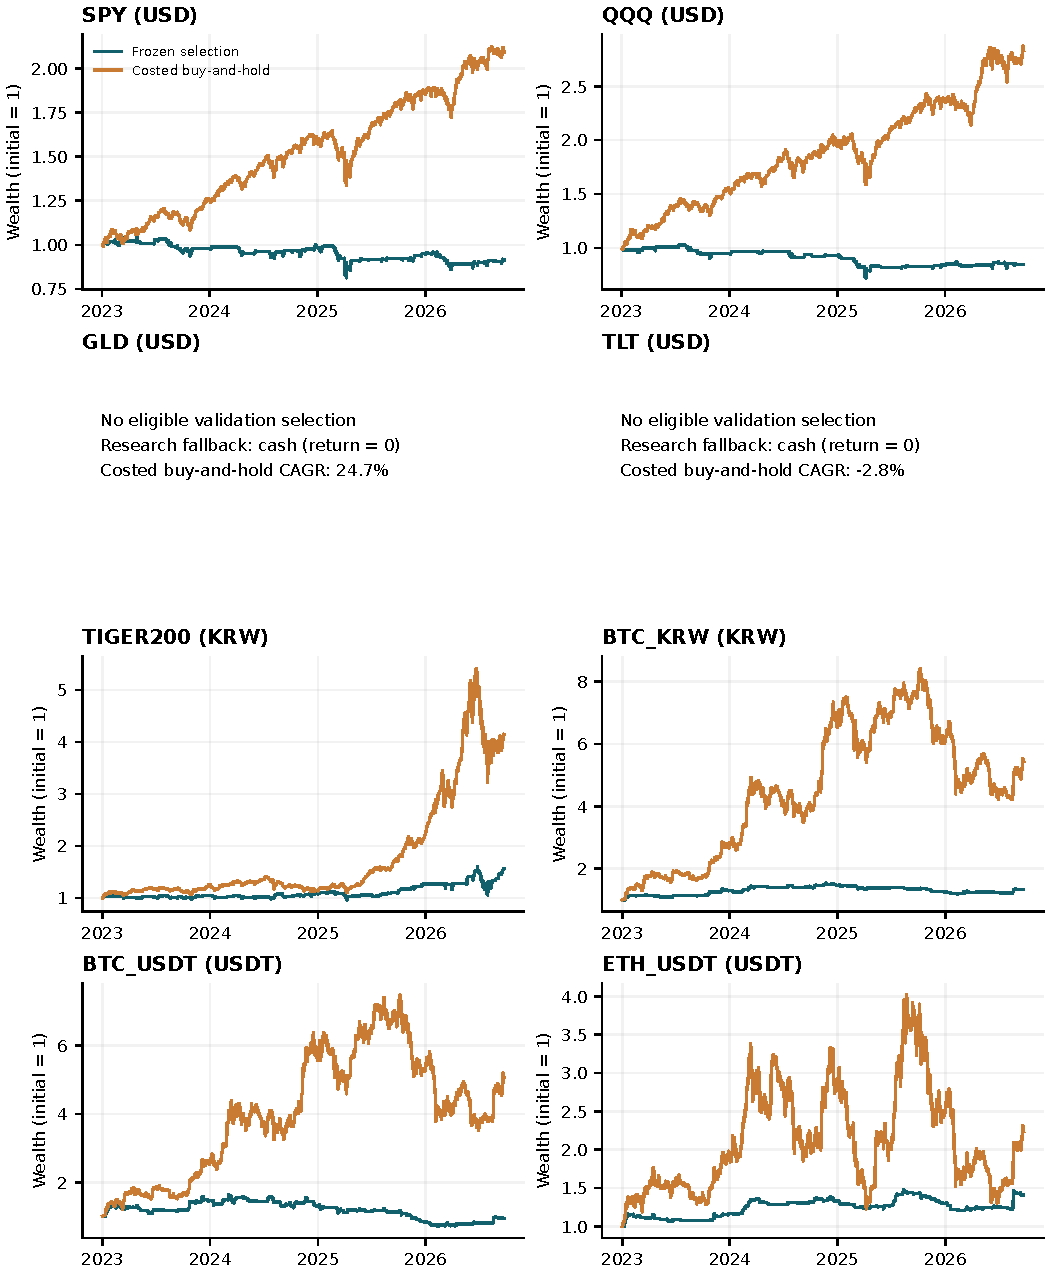
\includegraphics[width=\linewidth]{figures/selected_wealth.pdf}
\caption{검증 구간에서 고정한 선택의 회고적 이후 구간 자산곡선. 각 자산의 고유 표시 통화에서 최초 자산을 1로 정규화한다. 단순 보유도 동일 비용·시작·종료 규칙을 적용한다. 자산 간 곡선을 동일 원화 수익으로 합산할 수 없다.}\label{fig:wealth}
\end{figure}
\begin{figure}[p]\centering
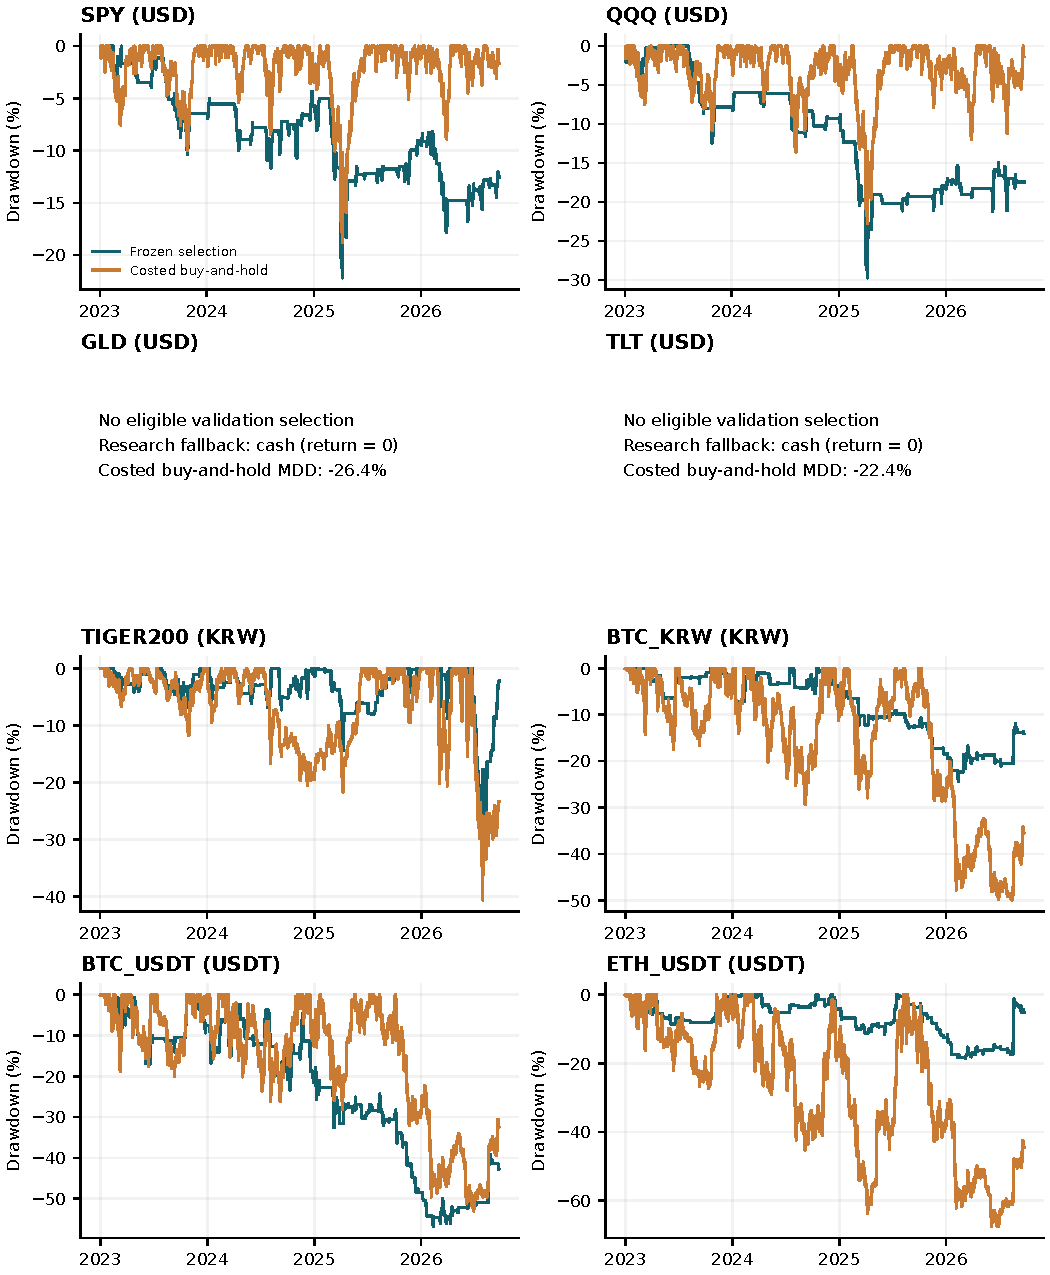
\includegraphics[width=\linewidth]{figures/selected_drawdowns.pdf}
\caption{같은 고정 선택과 단순 보유의 최대 고점 대비 낙폭 경로. 낮은 낙폭이 낮은 평균 노출에서 왔는지, 높은 수익률까지 동반하는지 구분해야 한다. 이 경로는 일봉 관측 사이의 최대 손실이나 실제 청산 가격을 보증하지 않는다.}\label{fig:drawdown}
\end{figure}
\begin{figure}[p]\centering
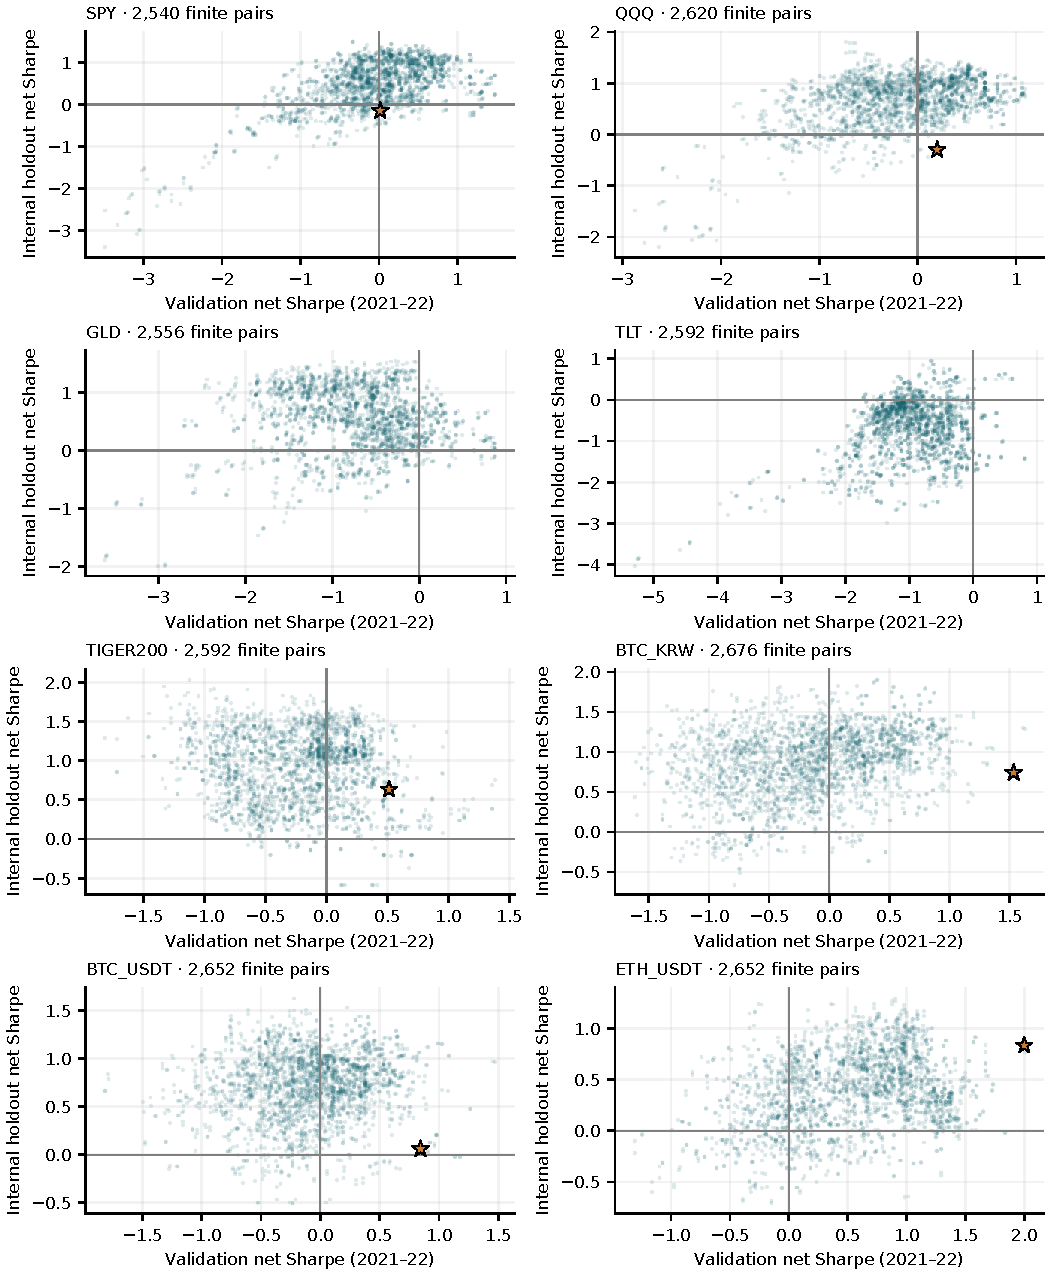
\includegraphics[width=\linewidth]{figures/selection_transfer.pdf}
\caption{모든 후보의 검증 구간과 회고적 이후 구간 샤프비율. 각 점은 설정 변형이고 서로 독립적이지 않다. 강조한 점만 검증 구간의 사전 규칙으로 선택되었다. 이후 구간 전체 분포는 선택을 고치기 위한 자료가 아닌 사후 진단이다.}\label{fig:transfer}
\end{figure}
\begin{figure}[p]\centering
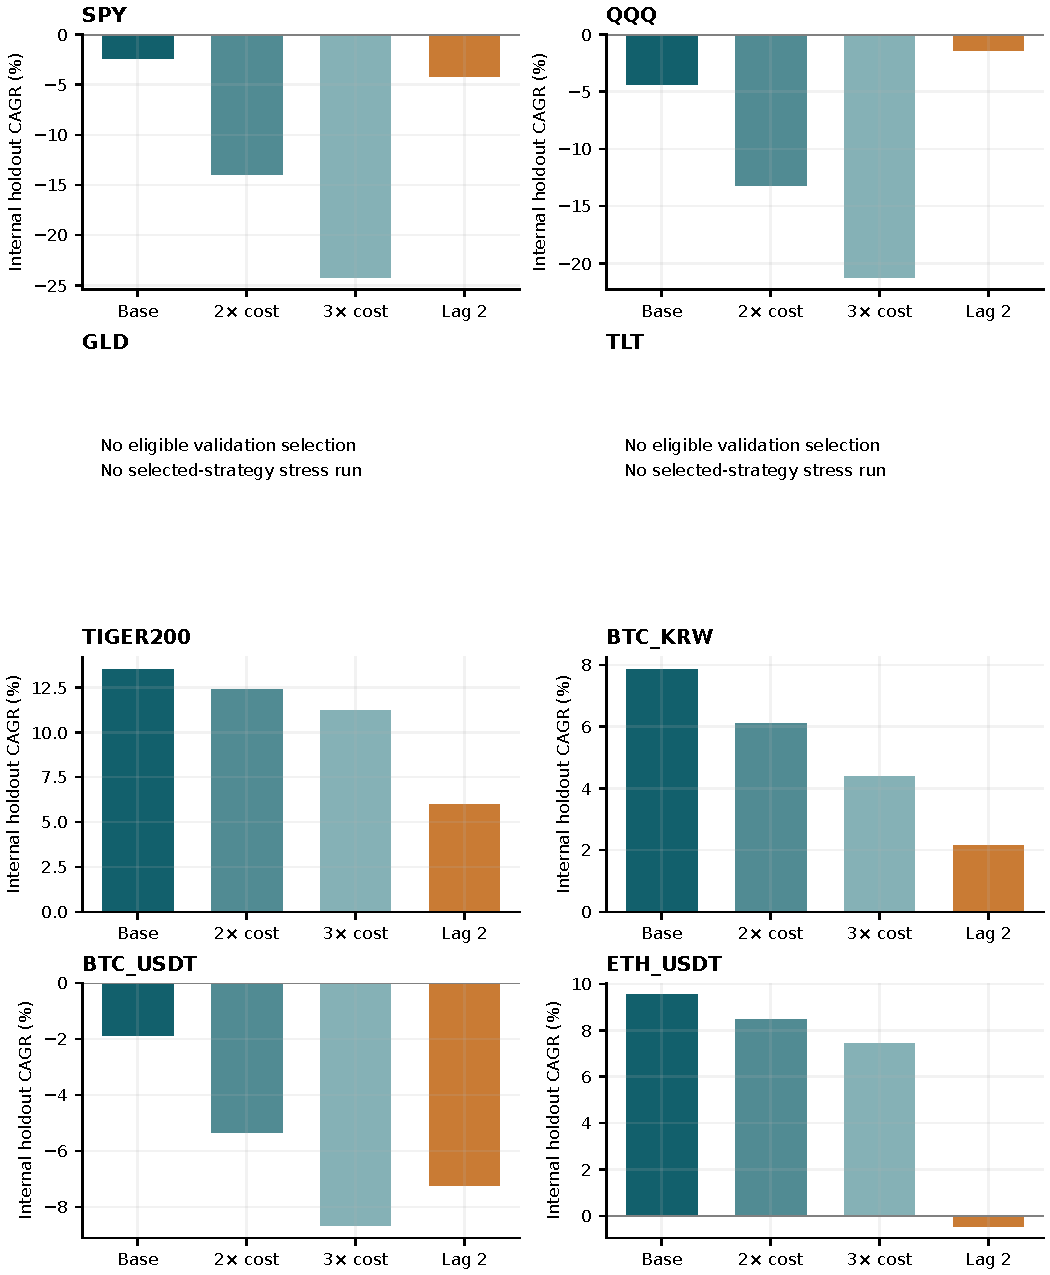
\includegraphics[width=\linewidth]{figures/cost_stress.pdf}
\caption{고정 선택의 비용·실행 지연 민감도. 기본 비용, 2배·3배 비용, 추가 한 봉 지연에서 이후 구간 연환산 성장률을 비교한다. 스트레스 결과를 이용한 재선택은 하지 않았다.}\label{fig:cost}
\end{figure}
\clearpage

\section{논의: 분석적으로 유의미한 것과 실행 가능한 것}
선택된 후보의 검증 샤프비율 중앙값은 0.68이고 이후 구간 중앙값은 0.35이다. 서로 다른 시장 상태·표본 길이·사후 선택이 함께 영향을 주므로 이 차이를 순수한 과최적화 효과라고 식별할 수 없다. 그림의 전체 후보 구름은 선택 구간의 성적이 다음 구간에 얼마나 불안정하게 전달되는지를 보여주는 진단이다.

선택 6개 중 단순 보유보다 관측 최대 낙폭이 작았던 것은 3개이다. 그 차이는 노출 축소의 대가와 함께 읽어야 하며 낮은 낙폭 자체가 예측 알파는 아니다. 기본 비용에서 평균수익이 양수였으나 2배 비용에서 비양수로 바뀐 선택은 1개이다. 그 밖에도 비용은 연속적으로 누적되므로 이 이분법만으로 비용 민감도가 없다고 결론내릴 수 없다. 추가 지연 실험은 시간 정렬의 취약성을 확인하지만 실제 거래소의 미체결·지연 분포를 추정한 것은 아니다.

암호자산 세 선택은 모두 5봉 이동평균·1\% 진입 여유·5봉 재조정이라는 방향 규칙을 공유한다. 그러나 비중 상한과 변동성 조절 정책이 다르며, 표시 통화와 시장의 일자 경계도 다르다. 따라서 원화 비트코인 선택과 USDT 비트코인 선택의 수익 차이를 거래소 우위, 환율 예측력 또는 통화 자체의 효과로 식별할 수 없다. 이를 묻는 후속 실험은 동일 노출 정책·동일 시점·환율 환산을 별도로 고정해야 한다.

많은 설정이 같은 구간에서 비슷한 성적을 내는 경우는 신호가 안정적이라는 가설을 제공할 수 있지만, 서로 닮은 설정을 독립 복제로 세면 안 된다. 반대로 매우 좁은 설정만 좋은 경우는 민감도 문제를 드러내지만 그것만으로 과최적화를 확정할 수도 없다. 본 보고서는 탐색의 규모, 계열별 분포, 고정 선택의 이동, 비용 민감도를 함께 남겨 이후의 독립 실험이 반증 가능한 대상을 갖도록 한다.

위험 관리의 목적이 낙폭 감소라면 평균 노출이 같은 정적 벤치마크, 하락기 노출, 여러 독립적 하락 사건에 대한 기여를 따로 고정해야 한다. 높은 샤프비율을 선택하고 나서 불리한 수익률 결과를 낙폭 목표의 성공으로 바꾸는 일은 허용하지 않는다. 이번의 기본 추론 벤치마크는 비용 차감 단순 보유이며, 보호형 전략의 별도 주장 검정은 후속 연구이다.

\section{제약과 후속 확인 실험}
첫째, 자료는 이미 연구된 생존 자산 캐시이며 매수·매도 호가, 거래량, 체결 기록이 없다. 빈티지와 캡처 시각이 충분하지 않으므로 현재 거래 가능성과 미시구조를 판단할 수 없다. 둘째, 신호는 종가 가격만으로 만들어져 가치·이익·금리·성장률 같은 거시·기초 변수를 직접 검정하지 않는다. 경제학은 가설과 해석의 틀이며 관측하지 않은 변수를 검증했다는 장식이 아니다.

이 여덟 자산은 상장폐지 자산을 포함한 당시 전체 투자 가능 집합이 아니다. 이번 Holm 보정은 선언한 자산별 검정에 대한 것이며, 자산 선정과 이미 진행된 모든 과거 탐색의 다중성을 소급하여 보정하지 않는다.

셋째, 자기금융 소수 수량 모형도 실제 계좌는 아니다. 거래소 최소 금액, 정수 주식, 제한가 미체결, 부분 체결, 세금, 환전, 결제, 외부 입출금이 빠져 있다. 달력과 통화가 다른 수익률을 단일 계좌 성과로 합산하려면 추가 정합성이 필요하다. 넷째, 일별 평가수익을 실현 순이익으로 바꿔 부르지 않는다. 실제 손익 정책에는 FIFO 원장, 완전한 수수료·환율·현금흐름, 서울 일자 경계, 첫날과 이전 이익 0인 날의 미지정 예산이 필요하다.

다섯째, 무손실 하한과 최소 수익 목표를 이 일봉 백테스트가 보증하지 않는다. 평가액과 하한의 동률은 곧 손실 초과가 아니지만 비용·갭·지연을 없애는 조건도 아니다. 목표와 위험 예산을 분리한 실행 정책은 독립적으로 시험해야 한다. 이번 보고서는 특정 계좌의 원금 보호 정책을 만족했다는 인증을 발급하지 않는다.

후속 확인에서는 지금 고정한 후보·가설을 변경하지 않고 새로 수집한 시점 정합적 자료를 축적하고, 실제 거래 규격에 맞춘 모의 주문·체결 모델을 붙여야 한다. 그때도 과거 성적이 좋은 후보를 추가하는 변경은 새로운 실험으로 기록한다. 실계좌 서명·활성화와 주문은 이 연구의 산출물이 아니며 별도 소유자 절차와 실행 검증을 요구한다.

\section{결론}
21,408개 자산·설정 조합을 동일한 선언 절차로 평가한 결과, 사전 고정 탐색 조건을 모두 만족한 선택은 0개였다. 이 연구의 기여는 많은 후보를 좋은 순서로 나열한 데 있지 않고, 경제적 가설과 매개변수 변형을 구별하고 비용·시차·선택편향·자료 재사용을 같은 평가 안에 드러낸 데 있다. 후속 결정은 공개된 후보·설정과 실패 조건을 유지한 채 새로운 자료와 실거래 규격을 이용해 확인해야 한다. 이번 결과만으로 자동주문을 활성화하거나 실현 이익·원금 보호를 보장할 근거는 없다.

\appendix
\section{재현성과 보조 자료}
계산 전 고정 커밋: \path{8e7c6c85c5ed3799a7cb6d4ac350ebdf57af1175}.\par
프로토콜 SHA256: \path{5b32f60cec5e893af9dd2ef685c369240ded00c846ca521990d0a7b3e9b38aff}.\par
자료 매니페스트 SHA256: \path{3a8646f403bd1d0417fe6b6aaeb3f98e3789d77d37d4886f59a7f4928b750697}.\par
선택 레지스트리 SHA256: \path{1fdb53bb4400270e72e3bc84346f0f16dbd5f907f483faa7ce7d0442c2316c3b}.\par
상대 경로 \path{docs/research/2026-10-31-strategy-lab/results/}에 \texttt{summary.json}, \texttt{run\_manifest.json}, \texttt{selection\_registry.json}, \texttt{candidates\_all.csv}, \texttt{selected\_daily.csv}와 USD 슬리브 보조 자료를 보관한다. 보고서 빌드는 \path{tools/build_strategy_paper.py}로 수행한다. 결과 파일과 생성기의 지문은 \texttt{paper/build\_manifest.json}에 기록한다.
\small\begin{longtable}{p{.16\linewidth}p{.76\linewidth}}
\caption{자산별 고정 후보와 설정}\\\toprule 자산 & 선택 내용 \\\midrule\endfirsthead
\toprule 자산 & 선택 내용 \\\midrule\endhead
SPY & \path{rsi_reversion-bd69fa14cdf69a80}\newline lookback=5, lower=30, upper=60\newline 재조정 1봉; 목표 상한 1.0; 변동성 목표 없음 \\[6pt]
QQQ & \path{rsi_reversion-30781661a965f9ab}\newline lookback=5, lower=20, upper=50\newline 재조정 1봉; 목표 상한 1.0; 변동성 목표 없음 \\[6pt]
GLD & 선택 없음: no\_eligible\_validation\_candidate \\[6pt]
TLT & 선택 없음: no\_eligible\_validation\_candidate \\[6pt]
TIGER200 & \path{rsi_reversion-93fcf01f24f5e330}\newline lookback=5, lower=40, upper=50\newline 재조정 1봉; 목표 상한 1.0; 변동성 목표 없음 \\[6pt]
BTC\_KRW & \path{sma-23835b7a8be46790}\newline band=0.01, lookback=5\newline 재조정 5봉; 목표 상한 0.5; 변동성 목표 없음 \\[6pt]
BTC\_USDT & \path{sma-6291e9eb728ab677}\newline band=0.01, lookback=5\newline 재조정 5봉; 목표 상한 1.0; 변동성 목표 없음 \\[6pt]
ETH\_USDT & \path{sma-227f25dc26ddfa3e}\newline band=0.01, lookback=5\newline 재조정 5봉; 목표 상한 1.0; 변동성 목표 15.0\% \\[6pt]
\bottomrule\end{longtable}\normalsize

전체 후보 CSV는 성적이 낮은 설정, 선택되지 않은 설정, 비용·이후 구간 지표를 포함한다. 데이터 목록은 원본 파일과 선택 행의 SHA256을 고정하고, 결과 생성기는 프로토콜·코드·자료 지문과 환경 정보를 남긴다. 보고서 생성기는 결과를 읽고 그림과 표를 만들 뿐 전략을 선택하거나 검정을 다시 수행하지 않는다.

\section{서지 검증 범위}
서지정보는 연결된 웹 도구로 출판사·저자·대학·공식 연구기관의 메타데이터와 접근 가능한 초록을 대조하였다. 일부 DOI 리디렉션이나 유료 원문은 열리지 않았으며, 접근하지 못한 전체 원문을 읽었다고 주장하지 않는다. 참고문헌은 가설과 방법의 출처이고, 기존 논문의 수익률을 이번 실험의 결과로 재사용하지 않았다. 항목별 확인 방식은 \texttt{paper/bibliography.json}에 보관한다.

\begin{thebibliography}{99}
\small\setstretch{1.08}
\bibitem{tsmom} Moskowitz, T. J.; Ooi, Y. H.; Pedersen, L. H. (2012). Time series momentum. \emph{Journal of Financial Economics}, 104(2), 228–250. DOI: \url{https://doi.org/10.1016/j.jfineco.2011.11.003}.

\bibitem{technical} Brock, W.; Lakonishok, J.; LeBaron, B. (1992). Simple Technical Trading Rules and the Stochastic Properties of Stock Returns. \emph{The Journal of Finance}, 47(5), 1731–1764. DOI: \url{https://doi.org/10.1111/j.1540-6261.1992.tb04681.x}.

\bibitem{contrarian} Lo, A. W.; MacKinlay, A. C. (1990). When Are Contrarian Profits Due to Stock Market Overreaction?. \emph{The Review of Financial Studies}, 3(2), 175–205. DOI: \url{https://doi.org/10.1093/rfs/3.2.175}.

\bibitem{volmanaged} Moreira, A.; Muir, T. (2017). Volatility-Managed Portfolios. \emph{The Journal of Finance}, 72(4), 1611–1644. DOI: \url{https://doi.org/10.1111/jofi.12513}.

\bibitem{crashes} Daniel, K.; Moskowitz, T. J. (2016). Momentum crashes. \emph{Journal of Financial Economics}, 122(2), 221–247. DOI: \url{https://doi.org/10.1016/j.jfineco.2015.12.002}.

\bibitem{white} White, H. (2000). A Reality Check for Data Snooping. \emph{Econometrica}, 68(5), 1097–1126. DOI: \url{https://doi.org/10.1111/1468-0262.00152}.

\bibitem{hansen} Hansen, P. R. (2005). A Test for Superior Predictive Ability. \emph{Journal of Business \& Economic Statistics}, 23(4), 365–380. DOI: \url{https://doi.org/10.1198/073500105000000063}.

\bibitem{holm} Holm, S. (1979). A Simple Sequentially Rejective Multiple Test Procedure. \emph{Scandinavian Journal of Statistics}, 6(2), 65–70. DOI: \url{https://doi.org/10.2307/4615733}.

\bibitem{kunsch} Künsch, H. R. (1989). The Jackknife and the Bootstrap for General Stationary Observations. \emph{The Annals of Statistics}, 17(3), 1217–1241. DOI: \url{https://doi.org/10.1214/aos/1176347265}.

\bibitem{neweywest} Newey, W. K.; West, K. D. (1987). A Simple, Positive Semi-definite, Heteroskedasticity and Autocorrelation Consistent Covariance Matrix. \emph{Econometrica}, 55(3), 703–708. DOI: \url{https://doi.org/10.2307/1913610}.

\bibitem{factorzoo} Harvey, C. R.; Liu, Y.; Zhu, H. (2016). … and the Cross-Section of Expected Returns. \emph{The Review of Financial Studies}, 29(1), 5–68. DOI: \url{https://doi.org/10.1093/rfs/hhv059}.
\end{thebibliography}
\end{document}
